\documentclass[11pt]{article}
\usepackage[letterpaper,top=0.72in,bottom=0.82in,left=0.86in,right=0.86in]{geometry}
\usepackage[T1]{fontenc}
\usepackage[utf8]{inputenc}
\usepackage{amsthm}
\usepackage{newtxtext,newtxmath}
\usepackage[final]{microtype}
\usepackage{setspace}
\setstretch{1.035}
\usepackage{parskip}
\setlength{\parindent}{1.12em}
\setlength{\parskip}{0.16em}
\usepackage{amsmath,mathtools,bm}
\usepackage{booktabs,tabularx,array,longtable}
\usepackage{xcolor}
\definecolor{inkblue}{HTML}{17385F}
\definecolor{deepblue}{HTML}{0D2742}
\definecolor{softblue}{HTML}{EEF4FA}
\definecolor{softgray}{HTML}{F5F6F7}
\definecolor{warmgray}{HTML}{6C727A}
\usepackage{tikz}
\usetikzlibrary{arrows.meta,positioning,calc,fit}
\usepackage{caption}
\captionsetup{font=small,labelfont=bf,labelsep=period}
\usepackage{titlesec}
\titleformat{\section}{\Large\bfseries}{\thesection.}{0.55em}{}
\titleformat{\subsection}{\large\bfseries}{\thesubsection.}{0.5em}{}
\titlespacing*{\section}{0pt}{2.1ex plus .4ex minus .2ex}{0.85ex}
\titlespacing*{\subsection}{0pt}{1.6ex plus .3ex minus .2ex}{0.55ex}
\usepackage{enumitem}
\setlist[itemize]{leftmargin=1.35em,itemsep=0.16em,topsep=0.25em}
\usepackage{mdframed}
\newmdenv[linewidth=0.65pt,linecolor=inkblue,backgroundcolor=softblue,roundcorner=2pt,
  skipabove=0.8em,skipbelow=0.55em,innerleftmargin=11pt,innerrightmargin=11pt,
  innertopmargin=8pt,innerbottommargin=8pt]{eurekabox}
\newmdenv[linewidth=0.55pt,linecolor=black!55,backgroundcolor=softgray,roundcorner=1pt,
  skipabove=0.6em,skipbelow=0.65em,innerleftmargin=10pt,innerrightmargin=10pt,
  innertopmargin=7pt,innerbottommargin=7pt]{formalbox}
\usepackage{hyperref}
\hypersetup{
  colorlinks=true,
  linkcolor=inkblue,
  citecolor=inkblue,
  urlcolor=inkblue,
  pdfauthor={Michael Zot},
  pdftitle={When Invisible Differences Stay Invisible: Machine-Certified All-Order Congruence for Temporal Reconstruction},
  pdfsubject={A Structural Path Compression certificate in the OpenAI Navier-Stokes correction architecture},
  pdfkeywords={Navier-Stokes, Structural Path Compression, Lean, formal verification, MeanClass, congruence, quotient}
}
\usepackage[nameinlink,noabbrev]{cleveref}
\usepackage{fancyhdr}
\pagestyle{fancy}
\fancyhf{}
\fancyhead[L]{\small\textsc{M. Zot}}
\fancyhead[R]{\small\textsc{When Invisible Differences Stay Invisible}}
\fancyfoot[C]{\small\thepage}
\renewcommand{\headrulewidth}{0.35pt}
\setlength{\headheight}{14pt}
\newtheoremstyle{highend}{0.8em}{0.8em}{\itshape}{}{\bfseries}{.}{0.6em}{}
\theoremstyle{highend}
\newtheorem{theorem}{Theorem}[section]
\newtheorem{corollary}[theorem]{Corollary}
\newtheorem{proposition}[theorem]{Proposition}
\theoremstyle{definition}
\newtheorem{definition}[theorem]{Definition}
\newtheorem{remark}[theorem]{Remark}

\newcommand{\MeanClass}{\mathrm{MeanClass}}
\newcommand{\Flat}{\mathrm{Flat}}
\newcommand{\Iinf}{\mathcal I_{\infty}}
\newcommand{\Tmap}{\mathcal T}
\newcommand{\repo}{\nolinkurl{openai/NavierStokesAndEuler}}
\newcommand{\commit}{\texttt{f9e8bc5b38b6...}}
\newcommand{\commitfull}{\nolinkurl{f9e8bc5b38b6e212696e8a30e3e91517af887bbd}}
\newcommand{\proofrepo}{\href{https://github.com/mikecreation/ZotBot/tree/main/research/navier-stokes-spc/temporal-closure}{research/navier-stokes-spc/temporal-closure}}

\begin{document}
\thispagestyle{empty}
\begin{center}
  \vspace*{0.30in}
  {\small\scshape Working Preprint \quad | \quad September 2026}\par
  \vspace{0.10in}
  {\fontsize{21}{25}\selectfont\bfseries
  When Invisible Differences Stay Invisible:\\[0.12em]
  Machine-Certified All-Order Congruence for\\
  Temporal Reconstruction in a Formal Navier--Stokes Architecture\par}
  \vspace{0.20in}
  {\large Michael Zot}\par
  \vspace{0.06in}
  {\small Independent Researcher}\par
  \vspace{0.045in}
  {\small Corresponding author: \href{mailto:mike@ZotBot.Ai}{mike@ZotBot.Ai}}\par
  \vspace{0.045in}
  {\footnotesize Public proof package: \proofrepo}\par
  \vspace{0.11in}
  \rule{0.74\textwidth}{0.45pt}\par
  \vspace{0.16in}
\end{center}

\begin{abstract}
Structural Path Compression (SPC) asks whether a proof can carry distinctions that are necessary for one representation of the argument but unnecessary for the future mathematics the proof must preserve. This note machine-certifies one precise test of that idea inside the 2026 OpenAI Navier--Stokes formalization.

The baseline library already proves a one-state filtration estimate for the temporal mean reconstruction: residual inputs in \(\MeanClass\,\alpha\) produce a radial increment in \(\MeanClass\,(\alpha+1)\) and angular/axial increments in \(\MeanClass\,\alpha\). The new contribution is not a stronger analytic estimate. It is the two-state congruence needed for compression: if two admissible states share the same reconstruction geometry and their relevant residual-source differences lie in \(\MeanClass\,\alpha\), then the differences of their temporal reconstructions obey the same grade transfer. Quantifying this statement over every real order \(A\) yields an all-order theorem: inputs invisible at every finite mean-filtration order remain invisible after temporal reconstruction.

The exact 598-line Lean module compiles against \repo\ at commit \commit\ using Lean 4.34.0-rc2. The certification run returned \texttt{TRUE\_LAKE\_EXIT\_CODE=0}; the source contains no \texttt{sorry}, \texttt{admit}, or custom \texttt{axiom}; and \texttt{\#print axioms} for both target declarations reports only \texttt{propext}, \texttt{Classical.choice}, and \texttt{Quot.sound}. The complete source, checksum, reproduction script, source crosswalk, recorded certification output, and CI recipe are published with this note.

The result closes one operator-level obligation in a larger proposed quotient-by-all-order-invisible-differences program. It does not establish full-cycle quotient closure, debt or rank closure, the full stage-free SPC theorem, or a new Navier--Stokes blowup theorem.
\end{abstract}

\noindent\textbf{Keywords.} Navier--Stokes; Structural Path Compression; Lean; formal verification; congruence; filtration; quotient dynamics; proof architecture.\\
\textbf{MSC 2020.} 35Q30; 03B35; 68V15; 68T15.\\
\textbf{Baseline formalization.} \repo, commit \commit.\\
\textbf{Public artifacts.} \proofrepo.

\clearpage
\section*{The result in one page}
\addcontentsline{toc}{section}{The result in one page}

\begin{eurekabox}
\textbf{Eureka.} Compression is not proved by deleting information. It is proved by showing that the future stays blind to what was deleted. If two states differ only by something no finite accuracy level can see, then every operator used after the compression must fail to resurrect that difference.
\end{eurekabox}
\noindent\textbf{Science underneath.}
For a fixed moving-strip datum \(s\), define all-order flatness by
\[
\Flat_s(f) \iff \forall A\in\mathbb R,\ \MeanClass_s^A(f).
\]
The certified theorem concerns the temporal reconstruction operator \(\Tmap\). If the theta- and axial-residual source differences are in \(\MeanClass_s^\alpha\), then
\[
\Delta \Tmap_r\in \MeanClass_s^{\alpha+1},\qquad
\Delta \Tmap_\theta\in \MeanClass_s^{\alpha},\qquad
\Delta \Tmap_z\in \MeanClass_s^{\alpha}.
\]
Therefore
\[
\Flat_s(\Delta \theta)\wedge \Flat_s(\Delta z)
\Longrightarrow
\Flat_s(\Delta \Tmap_r)\wedge \Flat_s(\Delta \Tmap_\theta)\wedge \Flat_s(\Delta \Tmap_z).
\]
The radial component is obtained one order better and then lowered from \(A+1\) to \(A\) using the baseline monotonicity theorem \texttt{mono\_exponent}.

\begin{eurekabox}
\textbf{Eureka.} The baseline theorem says, ``one input of grade \(A\) produces one output of grade \(A\).'' Compression needs a different statement: ``two inputs that are indistinguishable to grade \(A\) remain indistinguishable after the operator.'' That change from a one-state estimate to a two-state congruence is the bridge from ordinary bounds to quotient mathematics.
\end{eurekabox}
\noindent\textbf{Science underneath.}
The OpenAI source already contains \texttt{temporalIncrementState\_classes}. This note adds and certifies
\begin{center}
\nolinkurl{NavierStokes.VariableGaugeMean.temporalIncrementState_difference_classes}
\end{center}
and its all-order corollary
\begin{center}
\nolinkurl{NavierStokes.VariableGaugeMean.temporalIncrementState_flat_classes}.
\end{center}
No claim is made that the \(\alpha\mapsto(\alpha+1,\alpha,\alpha)\) analytic gain is new. The formal increment is the congruence theorem and its all-order closure statement.

\begin{eurekabox}
\textbf{Eureka.} A quotient becomes real one operator at a time. Every certified congruence removes one place where ``discarded'' information could have leaked back into the future.
\end{eurekabox}
\noindent\textbf{Science underneath.}
This paper closes only the temporal-reconstruction arrow. The larger target remains
\[
F(\Iinf)\subseteq \Iinf,
\]
for the complete reduced correction cycle. Debt and later cycle components remain separate obligations.

\tableofcontents
\clearpage

\section{The compression question becomes a congruence question}
\begin{eurekabox}
\textbf{Eureka.} A long proof can confuse ``how we got here'' with ``what the future still needs.'' SPC turns that philosophical suspicion into a falsifiable condition: erase a distinction, then ask every future consumer whether it notices.
\end{eurekabox}
\noindent\textbf{Science underneath.}
Let \(C_1,C_2\) be two admissible states and let \(Q\) retain only a proposed compressed representation. To make \(Q\) a valid state reduction for an update map \(F\), one needs a congruence implication
\[
Q(C_1)=Q(C_2)\quad\Longrightarrow\quad Q(F(C_1))=Q(F(C_2)),
\]
or the corresponding asymptotic/filtered equivalence. The present campaign uses the latter. Two states are identified when their difference lies at every finite requested order. The formal risk is that a downstream map could amplify or expose an all-order-invisible difference at some fixed finite order. A valid quotient requires ruling that out operator by operator.

The temporal mean reconstruction is one such operator. It consumes the residual sources that remain after earlier correction stages and produces a triple of mean increments. Before this work, the source library certified how one admissible source propagates through the temporal reconstruction. The missing object for the quotient program was a theorem about \emph{differences of two states} under the same reconstruction geometry.

\section{What the OpenAI formalization already proves}
\begin{eurekabox}
\textbf{Eureka.} The new theorem did not need a new estimate. The estimate was already there. What was missing was the right question.
\end{eurekabox}
\noindent\textbf{Science underneath.}
At the pinned commit, \texttt{NavierStokes/WeightedClasses.lean} defines
\[
\MeanClass(s,\alpha,f):=\mathrm{MemClass}\bigl(s,(n,x)\mapsto s.\zeta(x),\alpha,f\bigr),
\]
and proves monotonicity in the exponent:
\[
\mathrm{MemClass}_\alpha(f)\wedge \beta\le \alpha
\Longrightarrow \mathrm{MemClass}_\beta(f).
\]
The theorem is exposed as \texttt{mono\_exponent}.

In \texttt{NavierStokes/VariableGaugeMean.lean}, the baseline library defines \texttt{temporalIncrementState}; its angular component is the temporal inverse applied to the theta residual, while its radial and axial components are reconstructed through the stream potential built from the axial residual. The same file contains
\texttt{temporalIncrementState\_classes}, whose relevant conclusion is schematically
\[
\MeanClass_s^\alpha(\theta\text{-residual}),\ 
\MeanClass_s^\alpha(z\text{-residual})
\Longrightarrow
\begin{cases}
\MeanClass_s^{\alpha+1}(M_{T,r}),\\
\MeanClass_s^{\alpha}(M_{T,\theta}),\\
\MeanClass_s^{\alpha}(M_{T,z}).
\end{cases}
\]
That theorem is the analytic engine reused here.

\begin{formalbox}
\textbf{Source-level distinction.} The finite-grade exponents are not claimed as a newly discovered analytic mechanism. The new certified layer proves that the same operator is compatible with subtraction of two admissible states sharing the same fixed reconstruction parameters, and then packages that compatibility into an all-order congruence theorem.
\end{formalbox}

\section{The new machine-certified statements}
\begin{eurekabox}
\textbf{Eureka.} ``Small'' is not enough for a quotient. You need ``small at every order,'' and then you need the operator to preserve that invisibility forever. The all-order theorem is the first half of that sentence made executable.
\end{eurekabox}
\noindent\textbf{Science underneath.}
Fix the same slow region, radial geometry, moving-strip parameters, temporal index map, axial direction, context, and admissibility data for two states \(u_1,u_2\). Write
\[
\Delta\theta_n(z)=u_1.\mathrm{thetaResidual}(c,n,z)-u_2.\mathrm{thetaResidual}(c,n,z),
\]
\[
\Delta z_n(z)=u_1.\mathrm{axialResidual}(c,n,z)-u_2.\mathrm{axialResidual}(c,n,z).
\]

\begin{theorem}[Certified finite-grade congruence]\label{thm:finite}
If
\[
\MeanClass_s^\alpha(\Delta\theta),\qquad \MeanClass_s^\alpha(\Delta z),
\]
then the componentwise temporal-increment differences satisfy
\[
\MeanClass_s^{\alpha+1}(\Delta M_{T,r}),\qquad
\MeanClass_s^\alpha(\Delta M_{T,\theta}),\qquad
\MeanClass_s^\alpha(\Delta M_{T,z}).
\]
This is the compiled Lean declaration
\nolinkurl{NavierStokes.VariableGaugeMean.temporalIncrementState_difference_classes}.
\end{theorem}

\begin{corollary}[Certified all-order temporal closure]\label{cor:flat}
If
\[
\forall A\in\mathbb R,\quad
\MeanClass_s^A(\Delta\theta)\ \text{and}\ \MeanClass_s^A(\Delta z),
\]
then
\[
\forall A\in\mathbb R,\quad
\MeanClass_s^A(\Delta M_{T,r})\wedge
\MeanClass_s^A(\Delta M_{T,\theta})\wedge
\MeanClass_s^A(\Delta M_{T,z}).
\]
This is the compiled Lean declaration
\nolinkurl{NavierStokes.VariableGaugeMean.temporalIncrementState_flat_classes}.
\end{corollary}

\noindent The corollary applies \cref{thm:finite} at the arbitrary requested order \(A\). Angular and axial outputs are already in order \(A\). The radial output is in order \(A+1\), and the proof concludes with
\[
\texttt{hR.mono\_exponent (by linarith)}
\]
to downgrade \(A+1\) to \(A\). This is why the theorem is genuinely all-order and not the earlier, insufficient \(\alpha=0\) specialization encountered during development.

\section{Why the formal proof is more than writing ``linearity''}
\begin{eurekabox}
\textbf{Eureka.} The algebra is simple; the geometry is where a false shortcut could hide. ``Subtract the two formulas'' only works if both formulas really live on the same moving domain with the same support and reconstruction parameters.
\end{eurekabox}
\noindent\textbf{Science underneath.}
The proof is intentionally conservative. It does not invent a new temporal inverse or new class estimate. It transports subtraction through the exact machinery already used by the baseline theorem. The formal proof has five layers.

\subsection{Fourier inverse commutes with subtraction}
The helper \texttt{familyInverse\_sub} expands the family Fourier coefficient of \(f-g\), proves coefficient subtraction, and transports it through the directional inverse series using summability and \texttt{tsum\_sub}. This certifies the linearity used by the temporal inverse rather than treating it as an informal algebraic rewrite.

\subsection{Centered temporal inversion commutes with subtraction}
The helper \texttt{temporalAtIndex\_sub} combines torus-average subtraction, centering, the source-to-family map, and the previous Fourier inverse identity to obtain exact componentwise subtraction for the temporal inverse.

\subsection{The radial stream potential commutes with subtraction}
The helper \texttt{streamPotential\_sub} proves subtraction through the normalized weighted source and the compact/past integral representation. The proof carries the support and integrability obligations required by the source API.

\subsection{The moving-fiber bridge}
The moving geometry is the important proof-engineering boundary. The proof freezes the slow variable on the relevant fiber, applies the fixed-fiber subtraction identities, and returns to the moving domain using the existing fiber-locality theorems. Positivity of \(qLength\) is proved at the actual moving point used by the local argument. This is the part that prevents a superficially linear argument from silently comparing objects on mismatched domains.

\subsection{Reuse the existing filtration estimates}
Once the difference source is established as admissible, the proof calls the existing source theorems
\begin{itemize}
  \item \texttt{meanClass\_scaledTemporalStreamBeta},
  \item \texttt{meanClass\_temporalAtIndex\_moving},
  \item \texttt{meanClass\_temporalStreamGamma},
\end{itemize}
on the difference source. The new theorem therefore inherits the source library's analytic estimates rather than reproving them.

\section{The structural meaning: a local quotient certificate}
\begin{eurekabox}
\textbf{Eureka.} A compression is safe when erased information has nowhere to come back from. This theorem closes one return tunnel.
\end{eurekabox}
\noindent\textbf{Science underneath.}
Let
\[
\Iinf(s)=\{f:\forall A\in\mathbb R,\ \MeanClass_s^A(f)\}.
\]
For the temporal residual interface, \cref{cor:flat} gives the operator-level preservation law
\[
(\Delta\theta,\Delta z)\in \Iinf(s)\times\Iinf(s)
\Longrightarrow
\Delta \Tmap\in \Iinf(s)^3.
\]
This is precisely the kind of congruence needed if the eventual reduced dynamics are to descend through an all-order equivalence relation.

It does \emph{not} follow from this theorem alone that the full correction map respects \(\Iinf\). The remaining mean-debt, rank, residual-return, and full-cycle arrows must be certified separately. The point is narrower: temporal reconstruction is no longer a live obstruction to this quotient program under the theorem's hypotheses.

\begin{figure}[t]
\centering
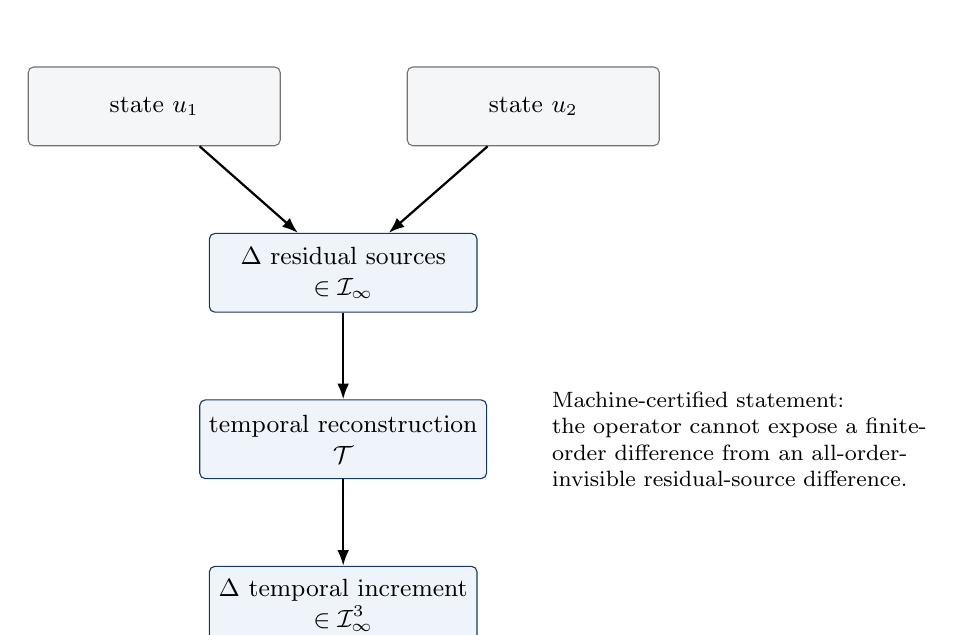
\begin{tikzpicture}[
  node distance=11mm and 16mm,
  every node/.style={font=\small,align=center},
  bx/.style={draw=inkblue,rounded corners=2pt,fill=softblue,minimum width=34mm,minimum height=10mm},
  gy/.style={draw=black!55,rounded corners=2pt,fill=softgray,minimum width=32mm,minimum height=10mm},
  ar/.style={-{Latex[length=2mm]},thick}
]
\node[gy] (u1) {state $u_1$};
\node[gy,right=of u1] (u2) {state $u_2$};
\node[bx,below=of u1,xshift=24mm] (din) {$\Delta$ residual sources\\$\in \Iinf$};
\node[bx,below=of din] (T) {temporal reconstruction\\$\mathcal T$};
\node[bx,below=of T] (dout) {$\Delta$ temporal increment\\$\in \Iinf^3$};
\draw[ar] (u1)--(din); \draw[ar] (u2)--(din); \draw[ar] (din)--(T); \draw[ar] (T)--(dout);
\node[right=7mm of T,text width=48mm,align=left,font=\footnotesize] {Machine-certified statement:\\the operator cannot expose a finite-order difference from an all-order-invisible residual-source difference.};
\end{tikzpicture}
\caption{The certified local congruence. The result is a statement about two-state differences under shared reconstruction geometry, not a new one-state gain estimate.}
\label{fig:congruence}
\end{figure}

\section{Machine certification and public reproducibility}
\begin{eurekabox}
\textbf{Eureka.} ``Lean proved it'' should not be a sentence readers are asked to trust. The proof object, the exact baseline, the checksum, and the commands should be public enough that the sentence can be replaced by a rebuild.
\end{eurekabox}
\noindent\textbf{Science underneath.}
The certification target is \texttt{NavierStokes/PandoraTemporalFlat.lean}, 598 lines. Its SHA-256 is
\begin{center}
\small\nolinkurl{13a6350607d73d101f107810986fcefbc73f5b41f308be8bf78c878f43e46c95}.
\end{center}
It was checked against \repo\ at the pinned commit
\begin{center}
\small\commitfull
\end{center}
with Lean 4.34.0-rc2. The recorded successful command was
\begin{verbatim}
set -o pipefail
lake build NavierStokes.PandoraTemporalFlat 2>&1 | tee /tmp/pandora-build.log
status=${PIPESTATUS[0]}
echo "TRUE_LAKE_EXIT_CODE=$status"
\end{verbatim}
and the recorded result was
\begin{verbatim}
Build completed successfully (3243 jobs).
TRUE_LAKE_EXIT_CODE=0
\end{verbatim}
The 3243 figure is the Lake job count of the targeted build; the project-side import closure of the target module comprised 157 NavierStokes modules. It is not the number of files in the full repository.

The final source audit found no \texttt{sorry}, \texttt{admit}, or custom \texttt{axiom}. \texttt{\#print axioms} for both target declarations reported only
\[
\{\texttt{propext},\ \texttt{Classical.choice},\ \texttt{Quot.sound}\}.
\]

\begin{formalbox}
\textbf{Public package.} The companion repository contains the exact Lean source, SHA-256 manifest, recorded certification output, axiom audit, source crosswalk, theorem-delta note, raw verification transcript, reproduction script, CI verifier, LaTeX source, and compiled PDF. The CI verifier is configured to commit its own build log, axiom output, exit code, and PASS status back into the public repository after a successful independent rerun, so the reproducibility layer does not stop at a prose record.
\end{formalbox}

\section{What changed during compilation}
The successful proof required four compiler-driven repairs to the supplied source. None weakened a theorem statement or changed the mathematical argument.
\begin{enumerate}[leftmargin=1.6em]
\item Open the \texttt{Topology} scope so the neighborhood notation \(\mathcal N\) / \texttt{nhds notation} elaborates.
\item In the first moving-fiber use of \texttt{temporalPotential\_sub\_on}, prove \texttt{qLength} positivity at the local point \texttt{p}, not at the outer point \texttt{z}.
\item Make the identical moving-point repair at the second occurrence.
\item Replace a syntactically failing direct rewrite by an explicit pointwise equality \texttt{hval} derived from the same eventual-equality fact, after beta reduction.
\end{enumerate}
The remaining compiler messages were non-fatal deprecation/linter warnings.

\section{What this proves, and what it does not}
\begin{eurekabox}
\textbf{Eureka.} The exciting statement is not ``we shortened Navier--Stokes.'' It is smaller and sharper: one piece of the proof can now be shown, mechanically, to forget an entire class of distinctions without letting them leak back into the future.
\end{eurekabox}
\noindent\textbf{Science underneath.}
The certified claim is exactly the finite-grade difference theorem plus the all-order temporal closure corollary. It establishes a local congruence property for temporal reconstruction under shared geometry and the stated admissibility hypotheses.

The following are \emph{not} established by this note:
\begin{itemize}
\item full reduced-cycle preservation of \(\Iinf\);
\item debt closure or rank closure;
\item existence of a complete quotient map \(\bar F:\mathcal C/\Iinf\to\mathcal C/\Iinf\);
\item the full stage-free SPC theorem from the companion manuscript;
\item a new Navier--Stokes blowup theorem;
\item absolute worldwide priority for the underlying functional-analytic fact.
\end{itemize}
These boundaries are part of the claim, not caveats added after the fact.

\section{Why this is useful even though the estimate already existed}
\begin{eurekabox}
\textbf{Eureka.} A bound tells you an object survives a calculation. A congruence tells you a distinction can be erased before the calculation. Those are different currencies of understanding.
\end{eurekabox}
\noindent\textbf{Science underneath.}
The source theorem \texttt{temporalIncrementState\_classes} answers a one-state question: given a source with a class bound, what class bound does its reconstruction satisfy? The new theorem answers a representation question: if two states differ only inside a specified negligible class, does the reconstruction distinguish them? Quotient constructions require the second form.

This distinction matters for proof architecture. If every consumer of a coordinate respects an equivalence relation, that coordinate need not remain independently represented merely because it appeared during one successful derivation. The mathematics can then be reorganized around equivalence classes or smaller interfaces. Conversely, failure of any one congruence theorem produces a precise witness that the proposed deletion was invalid. The same test therefore supports both compression and falsification.

\section{Relation to Structural Path Compression}
\begin{eurekabox}
\textbf{Eureka.} SPC began with a suspicious staircase: repeated stages looked fundamental because the proof walked them one by one. The deeper question is now sharper. Which distinctions are allowed to survive from one floor to the next?
\end{eurekabox}
\noindent\textbf{Science underneath.}
The companion SPC manuscript proposes replacing part of the repeated Section 9 chronology by an accuracy-indexed compiler once positive return estimates and source legality are established. The present theorem addresses a different but complementary issue that emerged from the later causal-state audit: whether candidate equivalence classes are invariant under the actual correction operators.

Thus Paper 1 and the present note should be read as two layers:
\[
\boxed{\text{Paper 1: recover a smaller generator from the successful path}}
\]
\[
\boxed{\text{Paper 2: certify that one deleted distinction stays deleted under a real operator}}
\]
The first is primarily architectural. The second is a machine-checked local preservation result.

\section{Next live theorem: debt closure}
\begin{eurekabox}
\textbf{Eureka.} Once one return tunnel is sealed, the frontier moves. The next question is not whether temporal reconstruction is safe; Lean has answered that. The next possible leak is debt.
\end{eurekabox}
\noindent\textbf{Science underneath.}
The next targeted implication in the all-order program is schematically
\[
\Flat(\Delta M)\wedge \Flat(\Delta \mathrm{Cov})\wedge \Flat(\Delta M_T)
\Longrightarrow
\Flat(\Delta \mathrm{Debt}).
\]
The source file \texttt{NavierStokes/GaugeDebtIncrement.lean} contains the relevant debt-update machinery. If debt closure and the remaining rank/cycle obligations are eventually certified, the stronger target becomes
\[
F(\Iinf)\subseteq\Iinf,
\]
which would permit a well-defined induced evolution on the corresponding quotient. That statement remains open in this note.

\section{Reproducibility map}
\begin{eurekabox}
\textbf{Eureka.} Reproducibility is strongest when every sentence of the form ``we checked X'' has a file or command sitting next to it. The public package is organized around that rule.
\end{eurekabox}
\noindent\textbf{Science underneath.}
The public package exposes the following artifacts directly:
\begin{itemize}
  \item \path{certification/PandoraTemporalFlat.lean}: exact 598-line source compiled in the certification run.
  \item \path{certification/SHA256SUMS.txt}: byte-level identity checks for the proof and publication artifacts.
  \item \path{certification/CERTIFICATION_RECORD.md}: environment, command, result, theorem names, and claim boundary.
  \item \path{certification/BUILD_RESULT.txt}: recorded successful Lake command/result.
  \item \path{certification/AXIOMS.txt}: recorded axiom audit for both target declarations.
  \item \path{certification/SOURCE_MAP.md}: exact baseline definitions and theorems reused from the pinned OpenAI tree.
  \item \path{certification/THEOREM_DELTA.md}: existing one-state estimate versus the new two-state and all-order statements.
  \item \path{certification/REVIEW_RESPONSE.md}: reviewer concern-to-fix crosswalk.
  \item \path{REPRODUCE.md} and \path{scripts/reproduce.sh}: independent rebuild and audit procedure.
  \item \path{.github/workflows/verify-navier-stokes-temporal.yml}: public CI verifier; successful reruns publish machine-generated logs under \path{certification/ci/}.
  \item \path{PUBLICATION_MANIFEST.md}: full skeptical-reader artifact manifest.
  \item \path{CLAIM_BOUNDARY.md}: explicit certification boundary.
\end{itemize}

\section{AI assistance disclosure}
AI systems were used as research tools for source retrieval, proof-dependency analysis, formal-proof drafting and debugging, adversarial checking, literature/prior-art search, and editorial drafting. The research direction, conceptual framework, selection and interpretation of claims, acceptance or rejection of proposed arguments, and publication decisions were determined by the author. The final theorem status reported here is tied to the public Lean artifact and reproducible build procedure, not to an AI-generated prose assessment.

\section{Conclusion}
\begin{eurekabox}
\textbf{Eureka.} The most useful thing a compression theorem can prove is not that a path is shorter. It is that the future has lost the ability to tell which path you took.
\end{eurekabox}
\noindent\textbf{Science underneath.}
The OpenAI formalization already supplied the analytic temporal reconstruction estimate. This work adds the two-state congruence and all-order closure required by the emerging SPC quotient program and checks both declarations in Lean against a pinned public baseline. The theorem is deliberately local, but its role is structural: temporal reconstruction cannot turn an all-order-invisible residual-source difference into a finite-order-visible temporal increment under the certified hypotheses.

That is one closed arrow. The larger quotient theorem remains to be earned arrow by arrow.

\begin{thebibliography}{9}
\bibitem{OpenAI2026NS}
OpenAI, \emph{Finite Time Blowup for Navier--Stokes}, 2026. Formal source repository: \url{https://github.com/openai/NavierStokesAndEuler}. Pinned baseline used here: commit \texttt{f9e8bc5b38b6e212696e8a30e3e91517af887bbd}.

\bibitem{Zot2026SPC}
M. Zot, \emph{Navier--Stokes: Recovering Minimal Structure from Representation-Induced Complexity}, working preprint, September 2026. \url{https://github.com/mikecreation/ZotBot/tree/main/research/navier-stokes-spc}.

\bibitem{Lean4}
L. de Moura and S. Ullrich, ``The Lean 4 Theorem Prover and Programming Language,'' in \emph{Automated Deduction -- CADE 28}, 2021.
\end{thebibliography}

\end{document}